\documentclass[12pt]{article}

\usepackage[active]{srcltx}

\usepackage{amsmath,amsfonts,amssymb,amsthm}
\usepackage{easybmat}
\usepackage{graphicx}
%\usepackage[hypertex]{hyperref}
%\usepackage[pdftex]{hyperref}
\usepackage{fancyhdr}
\usepackage{subfigure}

\usepackage{makeidx}
\makeindex

\theoremstyle{plain}
\newtheorem{theorem}{Theorem}
\newtheorem{property}[theorem]{Property}
\newtheorem{condition}[theorem]{Condition}
\newtheorem{proposition}[theorem]{Proposition}
\newtheorem{axiom}[theorem]{Axiom}
\newtheorem{lemma}[theorem]{Lemma}
\newtheorem{corollary}[theorem]{Corollary}
%%
% % Make numbering specific to the Appendix
% \newtheorem{Atheorem}{Theorem}[chapter]
% \newtheorem{Aproperty}[Atheorem]{Property}
% \newtheorem{Acondition}[Atheorem]{Condition}
% \newtheorem{Aproposition}[Atheorem]{Proposition}
% \newtheorem{Aaxiom}[Atheorem]{Axiom}
% \newtheorem{Alemma}[Atheorem]{Lemma}
% \newtheorem{Acorollary}[theorem]{Corollary}

% Make definitions non italicized
%\theoremstyle{definition}
\newtheorem{definition}[theorem]{Definition}
% Make numbering specific to the Appendix
%\newtheorem{Adefinition}[Atheorem]{Definition}
\newenvironment{defi}{\vskip0.2cm\addtocounter{theorem}{1}\par\noindent\bf Definition~\arabic{section}.\arabic{subsection}.\arabic{theorem}\rm.}{\hfill{$\circ$}\par\vskip0.25cm}


%% Example environment and counter.
\newcounter{cmpt_exercise}
\newenvironment{exercise}{\addtocounter{cmpt_exercise}{1}\vskip0.2cm\par\noindent\begin{small}\bf Exercise~\arabic{cmpt_exercise}\,\,\rm --}{\hfill{$\circ$}\end{small}\par\vskip0.25cm}
\newenvironment{problem}{\addtocounter{cmpt_exercise}{1}\vskip0.2cm\par\noindent{\Large\bf Problem~\arabic{cmpt_exercise}\,\,\rm --}}{\par\vskip0.25cm}


\newenvironment{example}{\vskip0.2cm\par\noindent\begin{small}\bf Example\,\,\rm --}{\hfill{$\diamond$}\end{small}\par\vskip0.25cm}
\newenvironment{remark}{\vskip0.2cm\par\noindent\begin{small}\bf Remark\,\,\rm --}{\hfill{$\circ$}\end{small}\par\vskip0.25cm}
%\newenvironment{aparte}[1]{\vskip0.2cm\par\noindent\begin{quote}\begin{small}\bf Apart\'e : #1\,\,\rm --}{\hfill{$\circ$}\end{small}\end{quote}\par\vskip0.25cm}
\newenvironment{aparte}[1]{\vskip0.3cm\par\begin{center}\begin{tabular}{|p{0.9\textwidth}|}\hline{\bf Apart\'e : #1}}{\\ \hline\end{tabular}\end{center}\par\vskip0.25cm}

\renewcommand{\labelenumi}{\roman{enumi})}
\renewcommand{\labelenumii}{\alph{enumii})}
\newcommand{\espv}{\vspace{.5\baselineskip}}
\def\IR{\mathbb{R}}
\def\IC{\mathbb{C}}
\def\IN{\mathbb{N}}
\def\IQ{\mathbb{Q}}
\def\IZ{\mathbb{Z}}
\def\rank{\textrm{rank }}
\def\Sp{\textrm{Sp }}
\def\Span{\textrm{Span }}
\def\Tr{\textrm{Tr }}
\def\D{\mathcal{D}}
\def\I{\mathcal{I}}
\def\U{\mathcal{U}}
\def\R{\mathcal{R}}
\def\Q{\mathcal{Q}}
\def\O{\mathcal{O}}
\def\Mn{\mathcal{M}_n}
\def\NN#1{\|#1\|}
\def\N3#1{|\!|\!|#1|\!|\!|}
\def\diag{\textrm{diag}}
\def\tr{\textrm{tr}}
\def\ker{\textrm{Ker }}

\def\M{\mathcal{M}}

\setlength{\textwidth}{17cm} 
\addtolength{\oddsidemargin}{-1.5cm}
\setlength{\textheight}{22cm}
\addtolength{\topmargin}{-2cm} 
\setlength{\headheight}{25.3pt}

%% Fancyhdr related stuff
\pagestyle{fancy}
\lhead{MATH 3820 -- Introduction Math. Model. -- Midterm -- Solutions}
\rhead{\thepage}
\cfoot{}

\usepackage[hang,small,bf]{caption2}
\setlength{\captionmargin}{20pt}

\makeatletter
\def\cleardoublepage{\clearpage\if@twoside \ifodd\c@page\else
\hbox{}
% \vspace*{\fill}
% \begin{center}
% This page intentionally contains only this sentence.
% \end{center}% Make numbering specific to the Appendix
\newtheorem{Atheorem}{Theorem}[chapter]
\newtheorem{Aproperty}[Atheorem]{Property}
\newtheorem{Acondition}[Atheorem]{Condition}
\newtheorem{Aproposition}[Atheorem]{Proposition}
\newtheorem{Aaxiom}[Atheorem]{Axiom}
\newtheorem{Alemma}[Atheorem]{Lemma}
\newtheorem{Acorollary}[theorem]{Corollary}

% \vspace{\fill}
\thispagestyle{empty}
\newpage
\if@twocolumn\hbox{}\newpage\fi\fi\fi}
\makeatother

%\author{Julien Arino}
%\address{University of Manitoba}
%\title{MATH 8430\\ Lecture Notes}
\title{University of Manitoba\\ Math 3820 -- Winter 2007}
\author{Midterm}
\date{Thursday, March 8, 2007}

\renewcommand{\abstractname}{Instructions}
%%%%%%%%%%%%%%%%
%%%%%%%%%%%%%%%%
%%%%%%%%%%%%%%%%
%%%%%%%%%%%%%%%%
%%%%%%%%%%%%%%%%
%%%%%%%%%%%%%%%%
\begin{document}

\maketitle
\thispagestyle{empty}
\begin{abstract}
This test is 1 hour and 15 minutes. It comprises 3 questions on 3 pages. Notes and calculators are allowed; computers are not allowed.
In marking, attention will be paid to the overall legibility of solutions; so detail and structure your answers.
\end{abstract}



\noindent
{\bf 1.a. (5 points)}
The variation in volume is given by
\[
V'=\textrm{input}-\textrm{output},
\]
that is,
\begin{equation}\label{eq:dV}
V'=r_{in}-r_{out},
\end{equation}
with initial condition $V(0)=500$.
\vskip0.5cm
\noindent
{\bf 1.b. (8 points)} 
Integrating \eqref{eq:dV} (a very simple integration here), we obtain
\[
V(t)=(r_{in}-r_{out})t+C.
\]
To find the integration constant, recall that the initial condition is $V(0)=500$. Therefore,
\[
V(0)=C=500,
\]
so the solution to \eqref{eq:dV} under the initial condition $V(0)=500$ is given by
\begin{equation}\label{eq:V}
V(t)=(r_{in}-r_{out})t+500.
\end{equation}

\vskip0.5cm
\noindent
{\bf 1.c. (8 points)}
We substitute the given values into \eqref{eq:V} (remembering that we have given the rates in minutes, so that 1 hour corresponds to $t=60$). This gives
\[
V(60)=(10-r_{out})60+500.
\]
Equating to 100, we obtain
\begin{align*}
(10-r_{out})60+500=100 &\Leftrightarrow 10-r_{out}=\frac{100-500}{60} \\
&\Leftrightarrow r_{out}=10+\frac{400}{60} \\
&\Leftrightarrow r_{out}\simeq 16.67
\end{align*}

\vskip0.5cm
\noindent
{\bf 1.d. (6 points)} 
All quantities are given in concentrations, so we need not bother about volume (although the latter is constant). Clearly, this functions like the chemostat, with the variation in concentration depending on the following parameters:
\[
C'=\textrm{concentration in the inflow}-\textrm{outflow}.
\]
Therefore,
\begin{equation}\label{eq:dC}
C'=r(t)S_0-r(t)C,
\end{equation}
with initial condition $C(0)=C_0$.

\vskip0.5cm
\noindent
{\bf 1.e. (5 points)}
We rewrite \eqref{eq:dC} as
\[
C'+r(t)C=r(t)S_0
\]
and use the result given. Therefore the general solution to \eqref{eq:dC} is given by
\begin{align*}
C(t) &= e^{-\int r(t)dt}\left(\int e^{\int r(t)dt}r(s)ds+K\right)
\end{align*}
To find the value of $K$, substitute $t=0$ in this solution, giving $C(0)=K$. Therefore,
\begin{align*}
C(t) &= e^{-\int r(t)dt}\left(\int e^{\int r(t)dt}r(s)ds+C_0\right).
\end{align*}


\vskip1cm
\noindent{\bf 2.a. (5 points)}
Suppose that $x_k\geq 0$. Then, since $a,b>0$, $ax_k\geq 0$ and $b+x_k>0$, so $x_{k+1}\geq 0$. For $x_0\geq 0$, $ax_0\geq 0$ and $b+x_0>0$, so that $x_1\geq 0$. Therefore, by induction, for $x_0\geq 0$, $x_t\geq 0$ for all $t$.
In fact, this can be tightened: it is clear, using the same reasoning, that $x_0=0$ implies that $x_t=0$ for all $t$, and $x_0>0$ implies that $x_t>0$ for all $t$.

\vskip0.5cm
\noindent{\bf 2.b. (8 points)} 
Let
\[
f(x)=\frac{ax}{b+x}.
\]
We seek $p$ such that $f(p)=p$. 
\begin{align*}
f(p)=p &\Leftrightarrow p=\frac{ap}{b+p} \\
&\Leftrightarrow
\left|
\begin{array}{l}
p=0\\
\textrm{or}\\
(b+p)p-ap=0
\end{array}
\right. \\
&\Leftrightarrow
\left|
\begin{array}{l}
p=0\\
\textrm{or}\\
(b-a+p)p=0
\end{array}
\right. \\
&\Leftrightarrow
\left|
\begin{array}{l}
p=0\\
\textrm{or}\\
p=a-b.
\end{array}
\right.
\end{align*}
Thus there are two fixed points, $p=0$ and $p=a-b$. 

\vskip0.5cm
\noindent{\bf 2.c. (10 points)}
The fixed point $p=0$ is always relevant. The fixed point $p=a-b$ is relevant only when $a>b$, since we have seen in {\bf 2.a} that solutions remain nonnegative for nonnegative initial conditions.

To study the stability of the fixed points, we study $|f'(p)|$. We have
\[
f'(x)=\frac{(b+x)a-ax}{(b+x)^2}=\frac{ab}{(b+x)^2}.
\]
Therefore, at $p=0$,
\[
|f'(0)|=\left|\frac{ab}{b^2}\right|=\left|\frac ab\right|=\frac ab,
\]
since $a,b>0$. Therefore, if $a>b$, $a/b>1$ and $0$ is repelling, whereas if $a<b$, $a/b<1$ and $0$ is attracting.

On the other hand, at $p=a-b$, we have
\[
|f'(a-b)|=\left|\frac{ab}{(b+a-b)^2}\right|=\left|\frac ba\right|=\frac ba,
\]
since $a,b>0$. Therefore, if $a<b$, then $b/a>1$ and $p=a-b$ is repelling, whereas if $a>b$, then $b/a<1$ and $p=a-b$ is attracting.

\vskip0.5cm
\noindent{\bf 2.d. (5 points)} 
To complete the picture, note that $p=a-b$ is the line parallel to the first bissectrix and through the point $a=b$. Therefore, we obtain the bifurcation diagram in Figure~\ref{fig:3} (in which the negative $p$ is plotted, even though it is not relevant. Such a bifurcation, where two equilibria exchange stability, is called a \emph{transcritical bifurcation}.
\begin{figure}[htbp]
\begin{center}
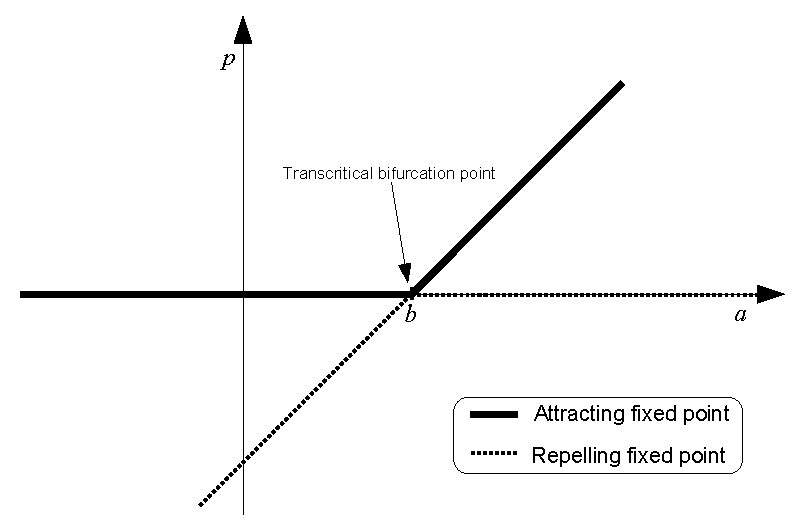
\includegraphics[width=0.75\textwidth]{fig2_midterm2007_solutions}
\caption{Bifurcation diagram for exercise {\bf 2.d}.}
\label{fig:3}
\end{center}
\end{figure}

\vskip0.5cm
\noindent{\bf 2.e. (5 points)}
We have
\begin{align*}
f^2(x) &= f(f(x)) \\
&= f\left(\frac{ax}{b+x}\right) \\
&= \frac{a\frac{ax}{b+x}}{b+\frac{ax}{b+x}} \\
&= \frac{a^2x}{b+x}\;\frac{b+x}{b(b+x)+ax} \\
&= \frac{a^2x}{b^2+(a+b)x}
\end{align*}
Points of period 2 satisfy $f^2(q)=q$. Clearly, here again $q=0$ is such a point (which is expected, since it is a fixed point). Then, dividing both sides of the equation $f^2(q)=q$ by $q$, we obtain
\[
\frac{a^2}{b^2+(a+b)q}=1,
\]
that is,
\[
q=\frac{a^2-b^2}{a+b}=\frac{(a-b)(a+b)}{a+b}=a-b.
\]
Therefore, the only period 2 points that we find are the fixed points. There are no period 2 points that are not fixed points (or, there are no points of least period 2).

\vskip1cm
\noindent{\bf 3.a. (8 points)}
The system becomes
\begin{equation}\label{eq:3}
\begin{aligned}
H' &= (b_H-d_H)H \\
F' &= -d_FF.
\end{aligned}
\end{equation}
These are two decoupled equations, which can thus be solved (easily) independently. We obtain
\begin{align*}
H(t) &= H_0 e^{(b_H-d_H)t} \\
F(t) &= F_0 e^{-d_F t}
\end{align*}
Since $d_F>0$, $\lim_{t\to\infty}F(t)=0$. If $b_H<d_H$, then $\lim_{t\to\infty}H(t)=0$. If $b_H=d_H$, $H(t)\equiv H_0$, the hare population remains constant. Finally, if $b_H>d_H$, then $\lim_{t\to\infty}H(t)=\infty$, the population explodes.


\noindent{\bf 3.b.}
In what follows, we will draw $H$ on the $x$-axis and $F$ on the $y$-axis.
To draw the nullclines easily, rewrite the system as
\begin{subequations}\label{eq:2}
\begin{align}
H' &= ((b_H-d_H) - \pi F)H \label{eq:2H}\\
F' &= (\sigma\pi H -d_F)F. \label{eq:2F}
\end{align}
\end{subequations}
We read the nullclines for $H$ in \eqref{eq:2H} by setting $H'=0$. We get the nullclines $H=0$ and $F=(b_H-d_H)/\pi$. 
Note that if $b_H-d_H<0$, then the second nullcline is not relevant.
Also, note that $H'>0$ if $(b_H-d_H)-\pi F>0$, that is, if $F<(b_H-d_H)/\pi$, that is, for $F$ below $F=(b_H-d_H)/\pi$. When $F$ is larger than $(b_H-d_H)/\pi$, $H'<0$.

The nullclines for $F$ are read in \eqref{eq:2F}. We find $F=0$ and $H=d_F/(\sigma\pi)$. Both these nullclines are always relevant. We have $F'>0$ if $\sigma\pi H-d_F>0$, that is, for $H>d_F/(\sigma\pi)$. In the contrary, if $H<d_F/(\sigma\pi)$, that is, left of the nullcline $H=d_F/(\sigma\pi)$, then $F$ is decreasing.

\noindent{\bf 3.c.}
Discuss the relevance (nonnegativity) and local stability of the equilibria, as a function of the relative values of $b_H$, $d_H$ and $d_F$, in the $\pi,\sigma>0$ case.

\end{document}